\section{Results}

We performed training with with several dataset configuration, but here we'll report only the most significant, however the reader may find implementation details, source code, trained models and log at \url{https://github.com/luca-m/emotime/}.

\subsection{Training Results}

Generalization performance are not formerly available due to the lack of a meaningful validation set\ref{res:issues}, so any generalization performance consideration should be taken as qualitative indications. Having said that we reported good performance in the detection of ``happiness'', ``anger'', ``disgust'', ``neutrality'' and ``surprise'', less effective is the detection of ``contempt'', ``sadness'' and ``fear''. We observed emotion detection happens on expression peeks which can be observed especially during face expression transitions, this behaviour could be caused by our current implementation of the binary classifiers: the SVM classifiers adopted provide a \emph{boolean information} about its prediction, an estimation of distance from the sample and the boundary hyperplane should enable a more gradual detection. 

We also observed that the \code{1vsAll} multiclass method provide more less noisy detections during a live web-cam session, \code{1vsAllExt} mode instead is able to always predict a valid state for each frame processed, but sometimes it result to be more unstable during the expression transition. 

\subsection{Issues}
\label{res:issues}

Here a brief discussion about problems and issues in general which remains unsolved due to the limited amount of time available for this class project.

\subsubsection*{Training Samples Number}

One of the main problem noticed during testing on arbitrary video or webcam is that detection of some emotions is not good as some other ones, a possible explanation rely on the limited amount of samples of the adopted dataset: some emotions have only 10/20 samples, which is certainly not a huge number.\\
Also the Cohn-Kanade Expression Database represent only the first step in several articles we have red, typically other dataset flanked to it (MMI, FERET, JAFFE, \ldots).

\subsubsection*{Validation Dataset}

The availability of a single, basic dataset did not give us the opportunity to calculate the confusion matrix on validation set for assessing generalization performance. 
%Also gaining access to datasets is not properly immediate: not automated registration, licence agreement and university affiliation are necessary.

\subsubsection*{Boosting Training Time}

The training time of multiple AdaBoost classifiers with $O(10^4)$ features is not negligible, it took more than a day to complete the whole training process. For this reason we chose to temporary skip the feature selection approach based on the boosting results and focus on SVM with linear kernel. 

This mean that our performance are not optimal because we may calculate some features which is actually not crucial in the decision process, nevertheless real-time performance are achieved.

\subsubsection*{Face Detector Side Effect}

We empirically noted that the face detector adopted for training and detection has side effect on generalization performance, a more formal discussion is not possible due to the lack of validation dataset availability. However we noted that using \code{haarcascade\_frontalface\_default} the face detection rate increase, but part of the ROI of the face is not useful for emotion detection due to the presence of part of background, hair and ears, giving worst generalization performance.

Using \code{haarcascade\_frontalface\_cbcl1} only the inner part of the face are detected, this lead to a lower face detection rate but the ROI results more dense of meaningful features. Since we resize ROI to a 48x48 rectangle, which are relatively small images, the effect of the trade-off described above is not negligible.

\subsection{Examples}

Following pictures represent screenshots captured during live test session with webcam and sample videos.

\begin{figure}
\centering
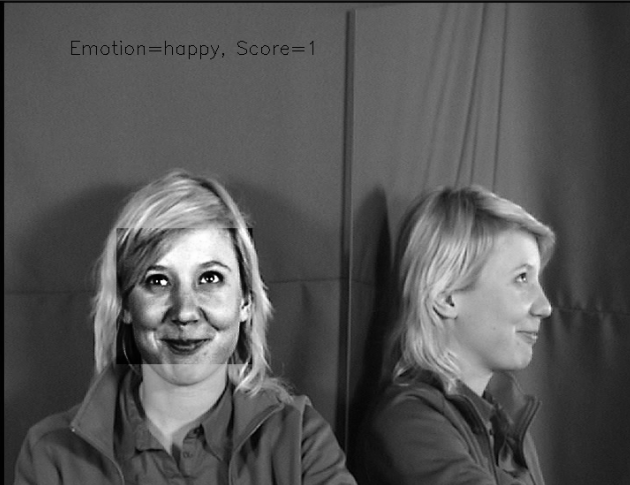
\includegraphics[width=7cm]{images/example_happy3.png}
\label{fig:example_happy3}
\caption{Happiness detection on a video from MMI dataset}
\end{figure}

\begin{figure}
\centering
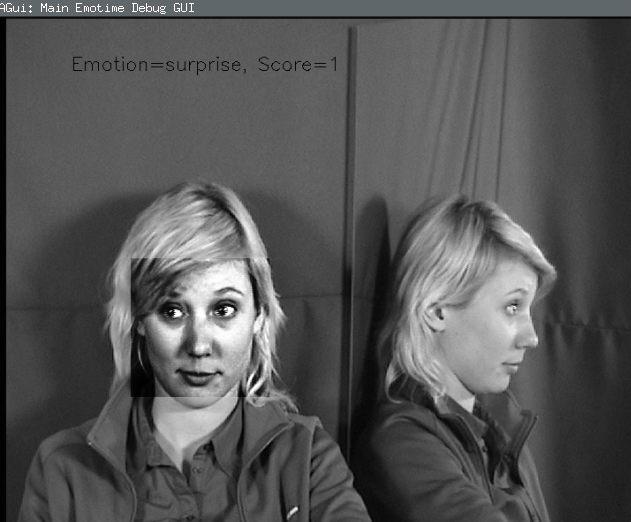
\includegraphics[width=7cm]{images/example_surprise.png}
\label{fig:example_surprise}
\caption{Surprise detection on a video from MMI dataset}
\end{figure}

\begin{figure}
\centering
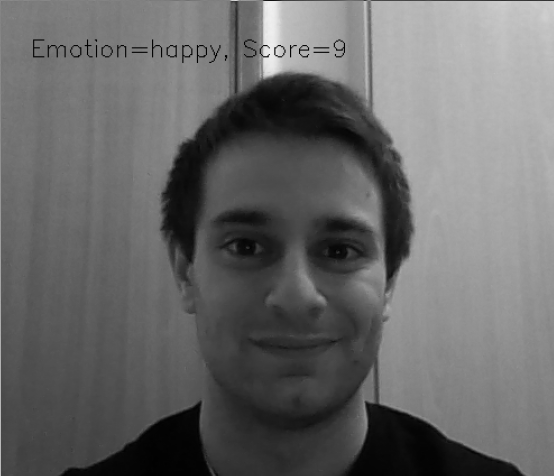
\includegraphics[width=7cm]{images/example_happy1.png}
\label{fig:example_happy1}
\caption{Happiness detection on live webcam capture}
\end{figure}

\begin{figure}
\centering
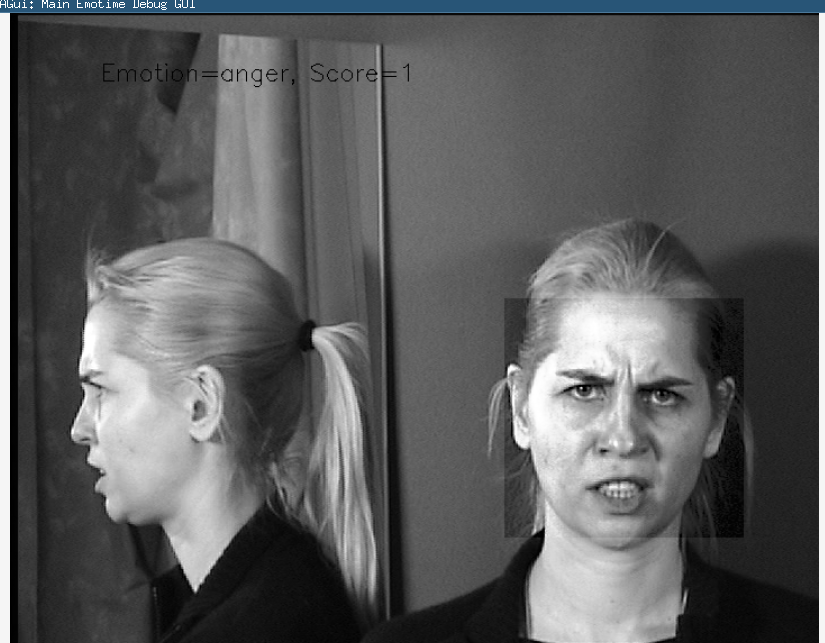
\includegraphics[width=7cm]{images/example_anger.png}
\label{fig:example_anger}
\caption{Anger detection on a video from MMI dataset}
\end{figure}

\begin{figure}
\centering
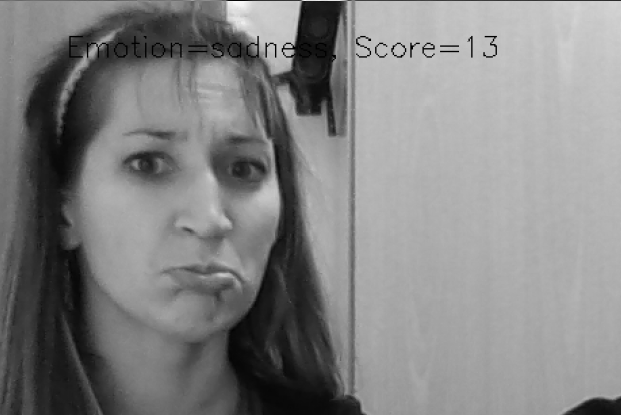
\includegraphics[width=7cm]{images/example_sad.png}
\label{fig:example_sad}
\caption{Sadness detection on live webcam capture}
\end{figure}

\begin{figure}
\centering
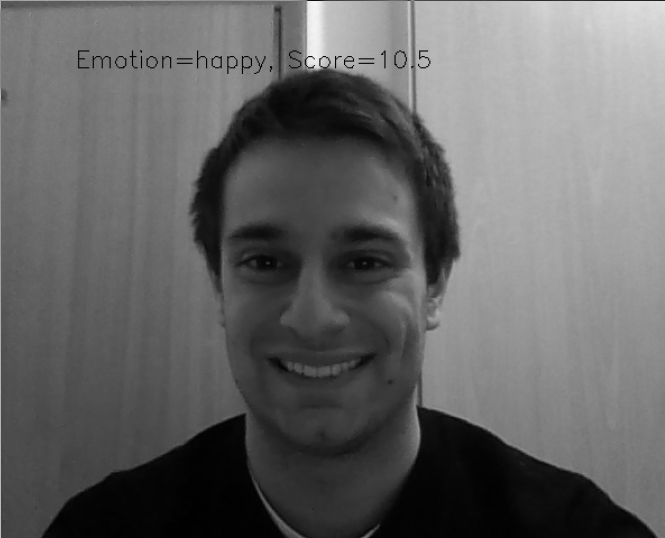
\includegraphics[width=7cm]{images/exampl_happy2.png}
\label{fig:exampl_happy2}
\caption{Happiness for happiness detection on live webcam capture}
\end{figure}

\begin{figure}
  \centering
  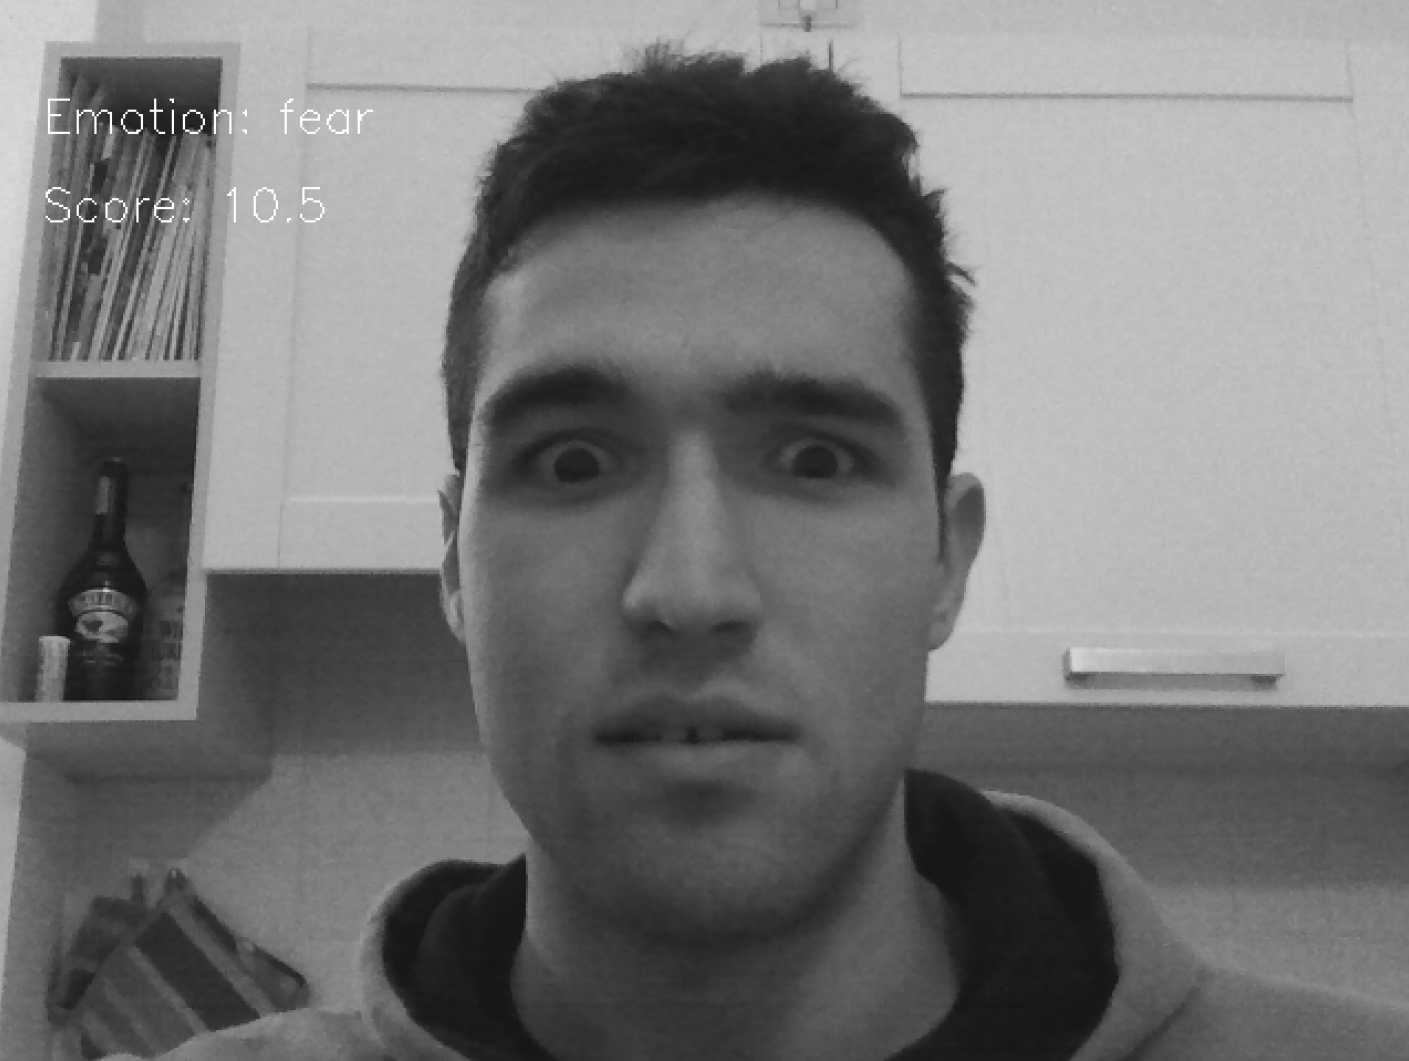
\includegraphics[width=7cm]{./images/db_fear.png}
  \caption{Fear detection on live webcam capture}
  \label{fig:exampl_fear}
\end{figure}

\begin{figure}
  \centering
  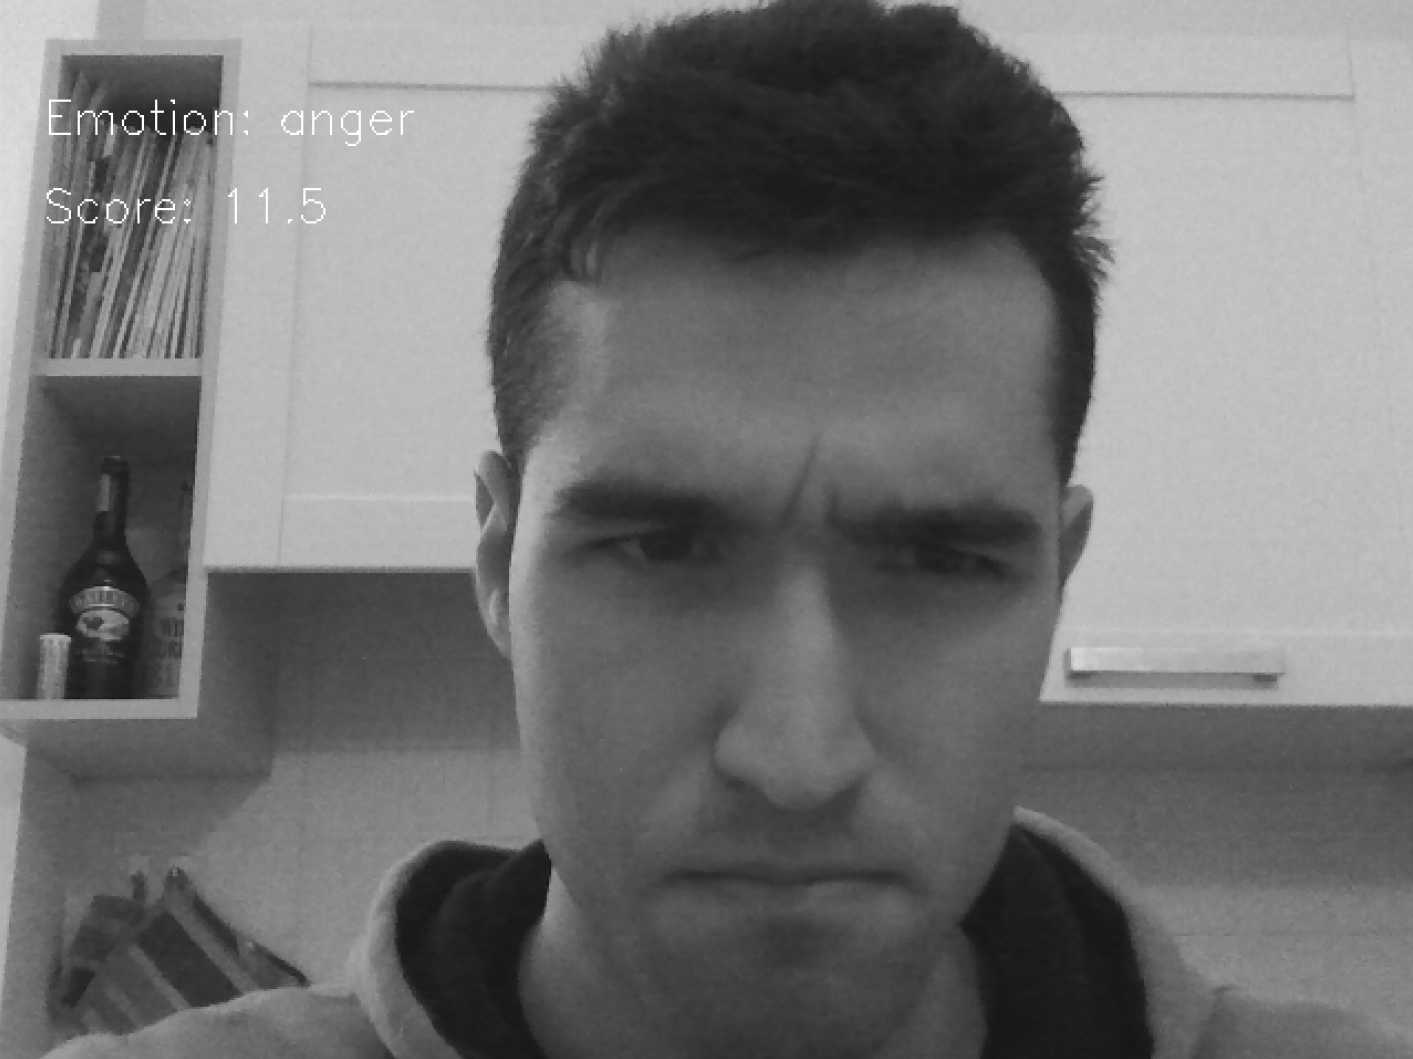
\includegraphics[width=7cm]{./images/db_anger.png}
  \caption{Anger detection on live webcam capture}
  \label{fig:exampl_anger}
\end{figure}

\begin{figure}
  \centering
  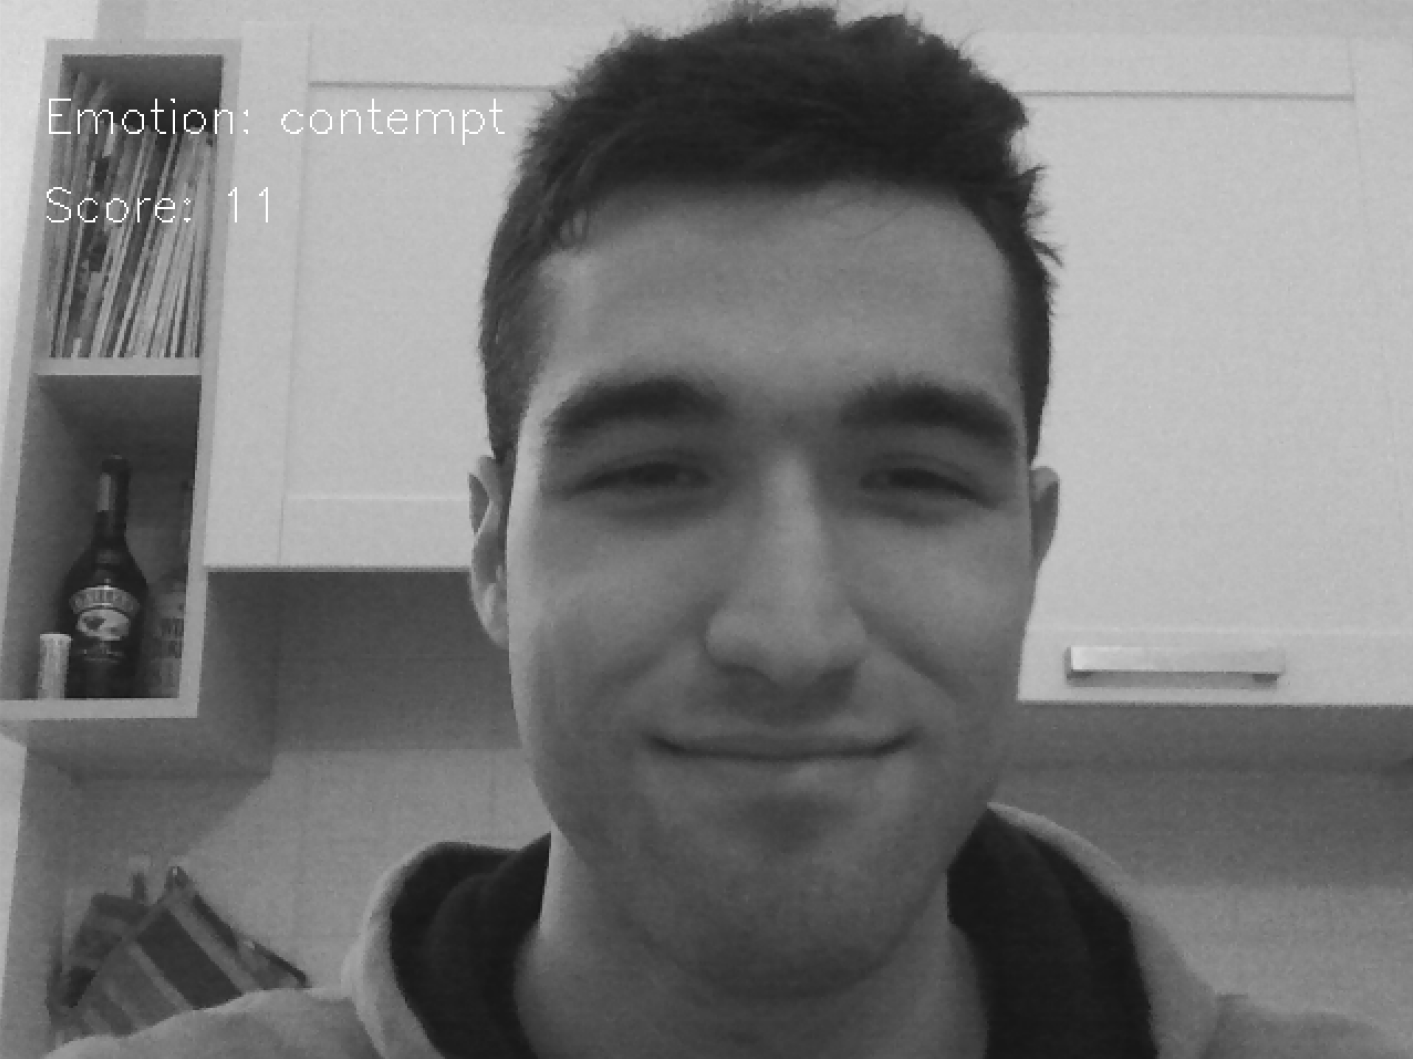
\includegraphics[width=7cm]{./images/db_contempt.png}
  \caption{Contempt detection on live webcam capture}
  \label{fig:exampl_contempt}
\end{figure}

\begin{figure}
  \centering
  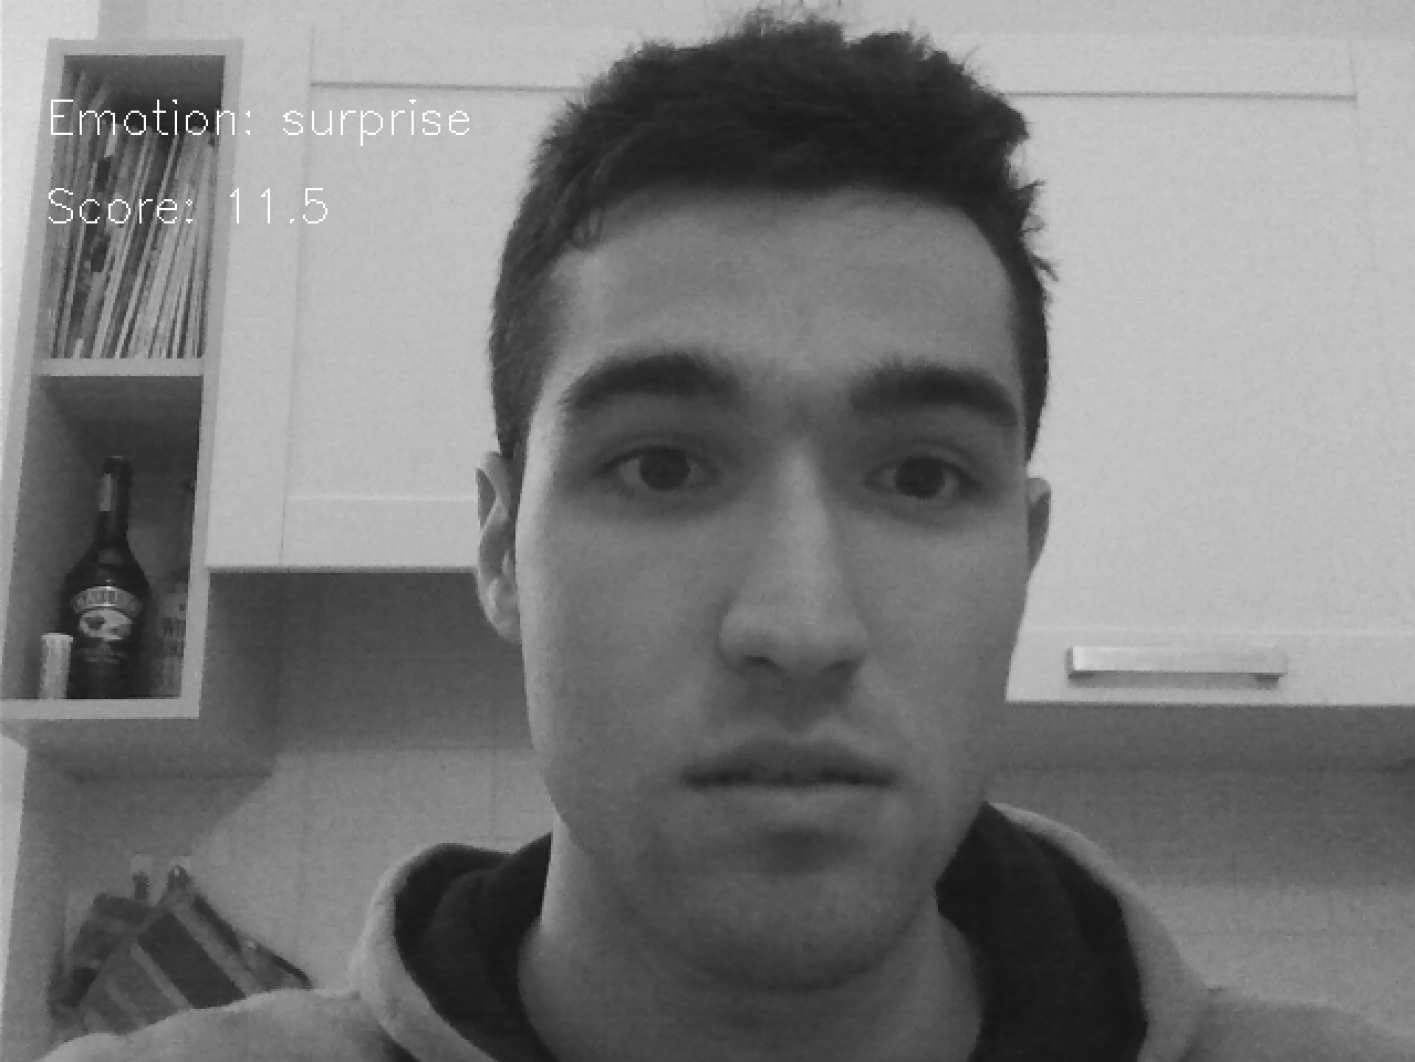
\includegraphics[width=7cm]{./images/db_surprise.png}
  \caption{Surprise detection on live webcam capture}
  \label{fig:exampl_surprise}
\end{figure}
\newpage
